%!TEX root = ../thesis.tex
%*******************************************************************************
%****************************** Second Chapter *********************************
%*******************************************************************************
\ifpdf
\graphicspath{{Chapter2/Figs/}}
\else
\graphicspath{{Chapter2/Figs/}}
\fi

\chapter{Scaling, Scale-Invariance and Self-Similarity}
In physics we observe a natural phenomena and try to understand it using the existing knowledge. To do this we need to assign numbers to the observable quantities. If we can express it in numbers only then we can say we have acquired some knowledge about that quantity. And if we cannot do this then our knowledge is not complete about that quantity. This reveals the fact that physics is all about observation and measurement of physical quantities with the desire to acquire some knowledge about it and then use that knowledge to predict something that is yet to observe. For example, Albert Einstein predicted the existence of gravitational waves in 1916 in his general theory of relativity and the first direct observation of gravitational waves was made on 14 September 2015 and was announced by the LIGO and Virgo collaborations on 11 February 2016. Now, in order to understand the observation of a natural or artificial phenomena we need some tools. Since here we are trying to understand phase transition, finite size scaling (FSS) hypothesis is a great tool for the investigation. In this chapter we will try to understand the fundamentals which is based on Buckingham $\pi$ theorem, self similarity and homogeneous functions.


\section{Dimensions of Physical Quantity}
	In order to express physical quantities in terms of numbers we need a unit of measurement, since a number times unit tells us how much the quantity is larger or smaller with respect to the unit. The units of measurement are described as fundamental and derivative ones. The fundamental units of measurement are defined arbitrarily in the form of certain standards, while the derivative ones are obtained from the fundamental units of measurement by virtue of the definition of physical quantities, which are always indications of conceptual method of measuring them. An example involving fundamental and derivative unit of measurement is velocity. Since velocity is measured by how much distance an object travels per unit time, the unit of velocity is the ratio of distance or length over time. It is expressed as $\left[v\right] = LT^{-1}$, where $L$ is the unit of length and $T$ is the unit of time. The unit of length and time are fundamental here and the unit of velocity is the derivative of these two. A system of units of measurement is a set of fundamental units of measurement sufficient to measure the properties of the class of phenomena under consideration. For example the \textit{CGS} system where length is measurement in terms of centimeter, mass is measured in terms of gram and the \textit{SI} system where the mass is measured in terms of kilogram, length is measured in terms of meter and in both system time is measured in terms of second.
	
	
	Dimension of physical quantity determines by what amount the numerical value must be changed if we want to go to another system of units of measurement. For instance, if the unit of length is decreased by a factor $L$ and the unit of time is decreased by a factor $T$, the unit of velocity is smaller by the factor of $LT^{-1}$ than the original unit, so the numerical value of velocity would scaled up by a factor of $LT^{-1}$ owing to the definition of equivalence.\\
	The changes in the numerical values of physical quantities upon passage from one systems of	units of measurement to another within the same class are determined by their dimensions. The	functions that determines the factor by which the numerical value of a physical quantity changes	upon transition from systems of unit of measurement to another system within a given class is	called the dimension function or, the dimension of that physical quantity.We emphasize that the	dimension of a given physical quantity is different in different classes of systems of units. For	example, the dimension of density $I$ in the $MLT$ class is $[\rho] = ML^{-3}$ whereas in the $FLT$ class it	is $[\rho] = F L^{-4}T^{-2}$ \cite{dimension_class_FLT, Sabbir}.
	
\section{Buckingham $\pi$ Theorem}
A part of physics is about modeling physical phenomenon. And while doing it, the first thing is to identify the relevant variables, and then relate them using known physical laws. For simple phenomenon this task is not hard since it involves deriving some quantitative relationship among the physical variables from the first principles. But when dealing with complex systems we need a systematic way of dealing with the problem of reducing number of parameters. In these situations constructing a model in a systematic manners with minimum input parameters that can help analyzing experimental results has been a useful method. One of the simplest way is based on dimensional analysis. Its function is to reduce a large number of parameters into a manageable set of parameters. Buckingham $\pi$ theorem is one of the most suitable and studied mathematical process to deal with this kind of problems.


Buckingham $\pi$ theorem describes dimensionless variables obtained from the power products of governing parameters denoted by $\Pi_1$, $\Pi_2$, $\ldots$ etc. When investigating a certain dimensional physical quantity (governed) that depend on other $n$ dimensional variables then this theorem provide us a systematic way to reduce the degrees of freedom of a function. Using this theorem we reduce a function of $n$ variables problems into a function of $k$ dimensionless variable problem if each of the $k$ dimensional variable of original $n$ variables can be expressed in terms of the $n-k$ dimensionally independent variable \cite{Buckingham1914}.


The relationship found in physical theories or experiments can always be represented in the form
\begin{equation}
a = f (a_1, a_2, \ldots, a_n)
\label{def:governed_governing}
\end{equation}
where the quantities $a_1, a_2, \ldots, a_n$ are called the governing parameters. It is always possible to classify the governing parameters $a_i$'s into two groups using the definition of the dependent and independent variables. Let the arguments $a_{k+1},\ldots,a_n$ have the independent dimensions and the dimensions of the arguments $a_1, a_2, \ldots, a_k$ can be expressed in terms of the dimensions of the governing independent parameters $a_{k+1}, \ldots, a_n$ in the following way
\begin{align}
	\left[a_1\right] &= \left[a_{k+1}\right]^{\alpha_1} 
	\ldots \left[a_n\right]^{\gamma_1} \nonumber\\
	\left[a_2\right] &= \left[a_{k+1}\right]^{\alpha_2} \ldots \left[a_n\right]^{\gamma_2}\\
	\vdots \\
	\left[a_k\right] &= \left[a_{k+1}\right]^{\alpha_k} \ldots \left[a_n\right]^{\gamma_k} \nonumber
\end{align}
The dimension of the governed parameter $a$ must also be expressible in terms of the dimensionally independent governing parameters $a_1, \ldots, a_k$ since $a$ does not have independent dimension and hence we can write
\begin{equation}
	\left[a\right] = \left[a_{k+1}\right]^{\alpha} \ldots \left[a_n\right]^{\gamma}
	\label{dimension_relation}
\end{equation}
Thus, there exist number $\alpha$, $\gamma$ such that \ref{dimension_relation} holds. We have set of governing parameters.
\begin{align}
	\Pi_1 &= \frac{a_1}{\left[a_{k+1}\right]^{\alpha_1} \ldots \left[a_{n}\right]^{\gamma_1}} \\
	\Pi_2 &= \frac{a_2}{\left[a_{k+1}\right]^{\alpha_2} \ldots \left[a_{n}\right]^{\gamma_2}} \\
	\vdots \\
	\Pi_k &= \frac{a_k}{\left[a_{k+1}\right]^{\alpha_k} \ldots \left[a_{n}\right]^{\gamma_k}}
\end{align}
and a dimensionless governed parameter
\begin{align}
\Pi 
&= \frac{a}{\left[a_{k+1}\right]^{\alpha} \ldots \left[a_n\right]^{\gamma}} \nonumber\\
&=\frac{f(\Pi_1, \ldots \Pi_k, a_{k+1}, \ldots, a_n)}{\left[a_{k+1}\right]^{\alpha} \ldots \left[a_n\right]^{\gamma}}
\label{dimensionless-pi-1}
\end{align}
The right hand side of equation \ref{dimensionless-pi-1} clearly reveals that the dimensionless quantity $\Pi$ is a function of $a_{k+1},\ldots,a_n,\Pi_1,\ldots,\Pi_k$, i.e.,
\begin{equation}
	\Pi \equiv F(a_{k+1}, \ldots, a_n, \Pi_1,\ldots,\Pi_k)
	\label{dimensionless-relation}
\end{equation}
The quantities $\Pi, \Pi_1,\ldots, \Pi_k$ are obviously dimensionless, and hence upon transition from one system of unit to another inside a given class their numerical values must remain unchanged. At the same time, according to the above, one can pass to a system of units of measurement such that any of the parameters of $a_{k+1}, \ldots, a_n$, say for example, $a_{k+1}$, is changed by an arbitrary factor, and the remaining ones are unchanged. Upon such transition the first argument of $F$ is unchanged arbitrarily, and all other arguments of the function remain unchanged as well as its value $\Pi$. Hence, it follows $\frac{\delta F}{\delta_{a_{k+1}}} = 0$ and entirely analogously $\frac{\delta F}{\delta_{a_{k+2}}} = 0, \ldots , \frac{\delta F}{\delta_{a_n}}=0$. Therefore, the relation \ref{dimensionless-relation} is in fact represented by a function of $k$ arguments and proves it is independent of $a_{k+1}, \ldots, a_n$, that is,
\begin{equation}
	\Pi = \Phi(\Pi_1, \ldots, \Pi_k)
	\label{eqn:pi-phi-dimensionless}
\end{equation}
and the function $f$ can be written in the following special form (by combining \ref{dimensionless-pi-1, dimensionless-relation,eqn:pi-phi-dimensionless})
\begin{equation}
f(a_1,\ldots,a_k,\ldots,a_n) = a^{\alpha}_{k+1} \ldots a^{\gamma}_n \Phi(\Pi_1, \ldots, \Pi_k)
\label{special_form}
\end{equation}
equation \ref{special_form} is known as the Buckingham $\Pi$ theorem. It constitutes one of the central statements in dimensional analysis and has great bearings on scaling theory. 
	\subsection{An Example}
	An explicit example using this theorem is needed for better understanding it's application. The simplest example that can describe basic features of Buckingham $\Pi$ theorem is the area of a right triangle and Pythagorean theorem. \\
	Consider a right triangle where three sides are of size $a,b$ and $c$ and for definiteness, the smaller of its acute angles $\theta$. Assume that we are to measure the area $S$ of the triangle. The area $S$ can be written in the following form
	\begin{equation}
		S=S(a,b,c)
	\end{equation}
	However, the definition of two governing parameters $a$ and $b$ can be expressed in terms of $c$ alone since we have
	\begin{equation}
		\left[a\right] \sim \left[c\right] \text{ and } 
		\left[b\right] \sim \left[c\right]
	\end{equation}
	and so is true for the governed parameter $S$ as we can write the dimensional relation $\left[S\right] \sim \left[c^2\right]$. We therefore can define two dimensionless parameters
	\begin{align}
		\Pi_1 = \sin \theta = a/c \\
		\Pi_2 = \cos \theta = b/c
	\end{align}
	and the dimensionless governed paremeter
	\begin{equation}
		\Pi = \frac{S}{c^2} = c^{-2} S(c\Pi_1, c\Pi_2,c) \equiv F(c, \Pi_1, \Pi_2)
	\end{equation}
	Now it is possible to pass from one unit of measurement to another system of unit of measurement within the same class and upon such transition the arguments $\Pi_1, \Pi_2$ of the function $F$ and the function itself remain unchanged. It implies that the function $F$ is independent of $c$ and hence we can write
	\begin{equation}
		\Pi = \phi(\Pi_1, \Pi_2)
	\end{equation}
	However, $\Pi_1$ and $\Pi_2$ both depends on the dimensionless quantity $\theta$ and hence we can write 
	\begin{equation}
		S = c^2 \phi(\theta)
		\label{universal-character-triangle}
	\end{equation}
	where the scaling function $\phi(\theta)$ is universal in character. In order to further capture the significance of equation \ref{universal-character-triangle} we rewrite it as
	\begin{equation}
		\frac{S}{c^2} \sim \phi(\theta)
	\end{equation}
	This result has far reaching consequences. For instance, consider that we have a right triangle of any arbitrary sides $a^\prime \neq a$, $b^\prime \neq b$ and $c^\prime \neq c$ but have the same acute angle $\theta$ as before. This can be ensured by choosing an arbitrary point on the hypotenuse of the previous triangle and drop a perpendicular on the base $b$. Consider that the area of the new triangle is $S^\prime$ yet we will have
	\begin{equation}
		\frac{S}{c^2} = \frac{S^\prime}{\left(c^\prime\right)^2}
	\end{equation}
	since the numerical value of the ratio of the area over the square of the hypotenuse depends on the angle $\theta$. It implies that if we plot the ratio of the area over the square of the hypotenuse as a function $\theta$ all the data points should collapse onto a single curve regardless of the size of the hypotenuse and the respective areas of the right triangle. In fact, the details calculation reveals that 
	\begin{equation}
		\phi(b/c) = \frac{1}{2} \sin \theta
	\end{equation}
	This data collapse implies that if two or more right triangles which have one of the acute angle identical then such triangles are similar. We shall see later that whenever we will find data collapse between two different systems of the same phenomenon	then it would mean that the corresponding systems or their underlying mechanisms are similar. Similarly, if we find that data collected from	the whole system collapsed with similarly collected data from a suitably chosen part of the whole system then we can conclude that part is similar to the whole, implying self-similarity. On the other hand, if we have a set of data collected at many different times for a kinetic system and find they all collapse onto a single curve then we can say that the same system at different times are similar. However, similarity in this case is found of the same system at different times and hence we may coin it as temporal self-similarity.
	\begin{figure}
		\centering
		\captionsetup[subfigure]{width=0.9\textwidth}
		\begin{subfigure}[t]{.45\textwidth}
			\centering
			\includegraphics[width=\linewidth]{{{area_vs_arm}}}
			\caption{$S$ vs $b$ graph. $b$ is the base of the triangle which is varied for a single $\theta$.}		
		\end{subfigure}
		\begin{subfigure}[t]{.45\textwidth}
			\centering
			\includegraphics[width=\linewidth]{{{data_collapse}}}
			\caption{$S/c^2$ vs $b/c$ graph. This each graph contains information about all triangle with a certain acute angle, meaning the entire graph contains information about every right triangle.}		
		\end{subfigure}
		\caption{Application of Buckingham $\Pi$ theorem in a right triangle}
		\label{fig:pi-theorem-and-pythagorean-triangle}
	\end{figure}
	
\section{Similarity and Self-Similarity}

	The concept of physical similarity is a natural generalization of the	concept of similarity in geometry. For instance, two triangles are similar	if they differ only in the numerical values of the dimensional parameters, i.e. the lengths of the sides, while the dimensionless parameters,	the angles at the vertices are identical for the two triangles. Analogously,	physical phenomena are called similar if they differ only in their numerical values of the dimensional governing parameters; the values of the	corresponding dimensionless parameters $\Pi_1, \ldots, \Pi_k$ are being identical.	In connection with this definition of similar phenomena, the dimensionless quantities are called similarity parameters.
	The term \textit{self-similarity} is, as the term itself suggests, a structure or process and a part of it appear to be similar to the whole when compared. This also means that a self-similar structure is infinite in theory. Therefore the fundamental principle of a self-similar structure is the repetition of a unit pattern on different scales. 
	
	
	\subsection{An example}
	At this point a real world example will be helpful. Suppose we need to build an airplane. Obviously it's a billion dollar project. If we try to build the airplane directly without first building a prototype then we will wasting time, money and man power. Because we can not build an actual working airplane without following certain steps. First we need to build a small-scale model of the airplane. Then we need to test the model for performance. If it is satisfying then we can start building a prototype using the knowledge obtained from the experimentation on the model. Here the model and the prototype are similar to each other. That's why this method works. Since only the dimensional parameters are scaled.
	
	
	\subsection{Diving Into Similarity}
	Let us consider two similar phenomena, one of which will be called the prototype and the other the model. For both phenomena there is some relation of the form
	\begin{equation}
		\alpha = f(a_1, a_2, a_3, b_1, b_2)
	\end{equation}
	where the function $f$ is the same for both cases by the definition of similar phenomena, but the numerical values of the governing parameters $a_1, a_2, a_3, b_1, b_2$ are different. Thus for prototype we have
	\begin{equation}
		\alpha_p = f(a_1^{(p)}, a_2^{(p)}, a_3^{(p)}, b_1^{(p)}, b_2^{(p)})
	\end{equation}
	 and for model we have
 	\begin{equation}
		 \alpha_m = f(a_1^{(m)}, a_2^{(m)}, a_3^{(m)}, b_1^{(m)}, b_2^{(m)})
	 \end{equation}
	where the index $p$ denotes quantities related to the prototype and the index $m$ denotes quantities related to the model. Consider that $b_1$ and $b_2$ are dependent variable and thus they are expressed in terms of $a_1, a_2, a_3$ in both model and prototype systems. Using dimensional analysis we find for both phenomena
	\begin{equation}
		\Pi^{(p)} = \Phi(\Pi_1^{(p)}, \Pi_2^{(p)})
	\end{equation}
	and
	\begin{equation}
		\Pi^{(m)} = \Phi(\Pi_1^{(m)}, \Pi_2^{(m)})
	\end{equation}
	where the function $\Phi$ must be the same for the  model and the prototype. By the definition of similar phenomena the dimensional quantities must be identical in both the cases such as in the prototype and in the model, i.e.,
	\begin{align}
		\Pi_1^{(m)} = \Pi_1^{(p)} \\
		\Pi_2^{(m)} = \Pi_2^{(p)} 
	\end{align}
	It also follows that the governed dimensionless parameter satisfies
	\begin{equation}
		\Pi^{(m)} = \Pi^{(p)}
	\end{equation}
	Returning to dimensional variables, we get from the above equation
	\begin{equation}
		a_p = a_m \left(\frac{a_1^{(p)}}{a_1^{(m)}}\right)^{q_1} \left(\frac{a_2^{(p)}}{a_2^{(m)}}\right)^{q_2} \left(\frac{a_3^{(p)}}{a_3^{(m)}}\right)^{q_3}
	\end{equation}
	which is a simple rule for recalculating the results of measurements on the similar model for the prototype, for which direct measurement may be difficult to carry out for one reason or another.\\
	The conditions for similarity of the model to the prototype-equality of the similarity parameters $\Pi_1, \Pi_2$ for both phenomena show that it is necessary to choose the governing parameters $b_1^{(m)}, b_2^{(m)}$ of the model as to guarantee the similarity of the model to the prototype
	\begin{equation}
		b_1^{(m)} = b_1^{(p)} \left(\frac{a_1^{(m)}}{a_1^{(p)}}\right)^{\alpha_1}
		\left(\frac{a_2^{(m)}}{a_2^{(p)}}\right)^{\beta_1}
		\left(\frac{a_3^{(m)}}{a_3^{(p)}}\right)^{\gamma_1}
	\end{equation}
	and 
		\begin{equation}
	b_2^{(m)} = b_2^{(p)} \left(\frac{a_1^{(m)}}{a_1^{(p)}}\right)^{\alpha_2}
	\left(\frac{a_2^{(m)}}{a_2^{(p)}}\right)^{\beta_2}
	\left(\frac{a_3^{(m)}}{a_3^{(p)}}\right)^{\gamma_2}
	\end{equation}
	whereas the model parameters $a_1^{(m)}, a_2^{(m)}, a_3^{(m)}$ can be chosen arbitrarily. The simple definitions and statements presented above describe the entire content of the theory of similarity.
	
	
	\subsection{Self-Similarity}
	A system is called self-similar	When a small part of the system is similar to the whole system. A self similar structure is created by repetition of a unit pattern or a simple rule over different size scales \cite{Mandelbrot1983}. Although the term "self-similarity" itself is explanatory, some example gives better insight.
	
	\begin{figure}
		\centering
		\captionsetup[subfigure]{width=0.9\textwidth}
		\begin{subfigure}[t]{.45\textwidth}
			\centering
			
\includegraphics[width=7.5cm]{self-similarity/cauliflower.jpg}
			\caption{A cauliflower}
		\end{subfigure}
	%	\begin{subfigure}{.5\textwidth}
	%		
\includegraphics[width=.5\linewidth]{self-similarity/cauliflower_many.jpg}
	%		\caption{Many cauliflower}
	%	\end{subfigure}
		\begin{subfigure}[t]{.45\textwidth}
			\centering
			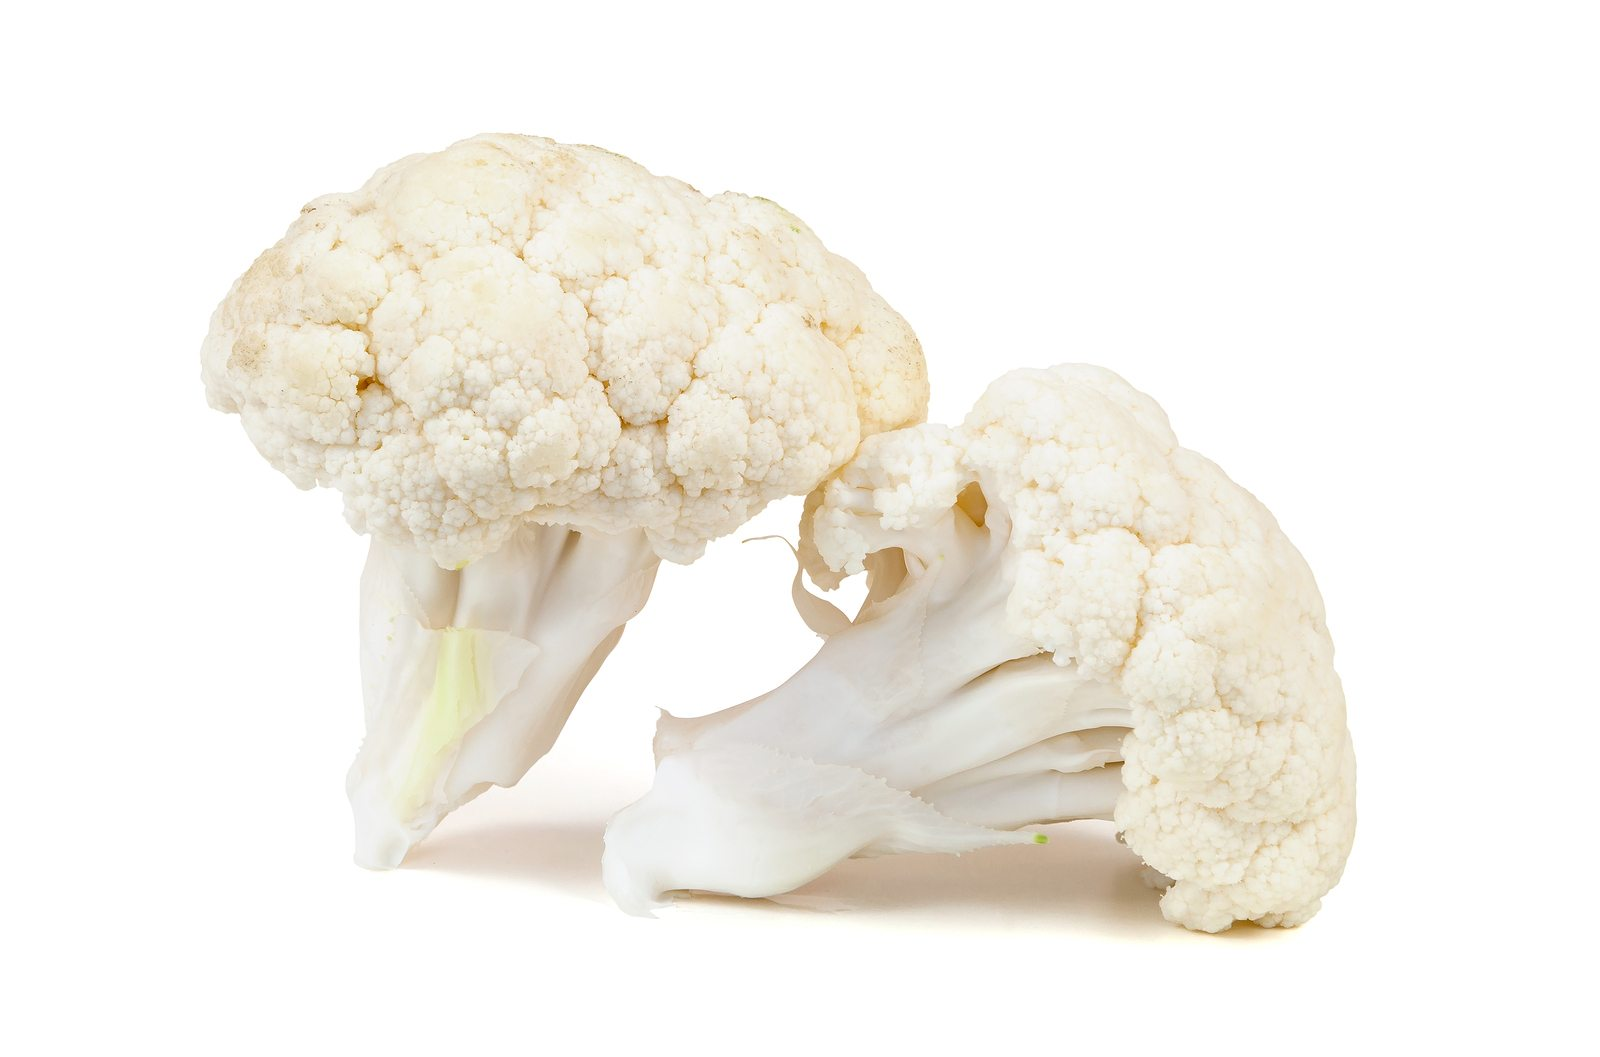
\includegraphics[width=7.5cm]{self-similarity/cauliflower_disected}
			\caption{Disection of cauliflower}
		\end{subfigure}
		\caption{Self-Similarity in Cauliflower}
		\label{fig:cauliflower-self-similarity}
	\end{figure}
	
	The cauliflower head contains branches or parts, which	when removed and compared with the whole found to be very much	the same except it is scaled down. These isolated branches can again	be decomposed into smaller parts, which again look very similar to the	whole as well as of the branches. Such self-similarity can easily be carried through for about three to four stages. After that the structures are	too small to go for further dissection. Of course, from the mathematical	point of view the property of self-similarity may be continued through	an infinite stages though in real world such property sustain only a few	stages \ref{fig:cauliflower-self-similarity}.
	
	\begin{figure}
		\centering
		\begin{tabular}{cc}
			% Requires \usepackage{graphicx}
			\begin{subfigure}{.6\textwidth}
				
\includegraphics[width=60mm,height=50mm]{self-similarity/leaf.jpg}
				\caption{Leaf}		
			\end{subfigure}
			&
			\begin{subfigure}{.6\textwidth}
				
\includegraphics[width=60mm,height=50mm]{self-similarity/snowflake.jpg}
				\caption{Snowflake}		
			\end{subfigure}
			\\
			\begin{subfigure}{.6\textwidth}
				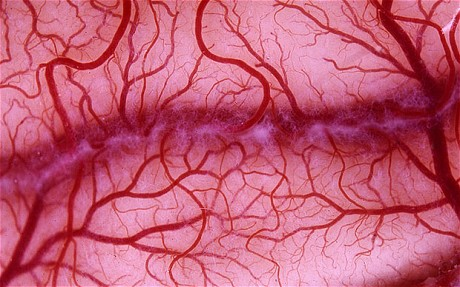
\includegraphics[width=60mm,height=50mm]{self-similarity/Blood_vessels.jpg}
				\caption{Blood vessel}		
			\end{subfigure}
			&
			\begin{subfigure}{.6\textwidth}
				
\includegraphics[width=60mm,height=50mm]{self-similarity/leafless-tree.jpg}
				\caption{Leafless Tree}		
			\end{subfigure}
			\\
		\end{tabular}
		
		\caption{Self-Similarity examples}
		\label{fig:example-self-similarity}
	\end{figure}


	There are plenty of other examples of self similarity in nature. Snowflakes exhibit self-similar branching patterns \ref{fig:example-self-similarity}. The growth in aggregating colloidal particles are statistically self-similar. A leafless tree branches \ref{fig:example-self-similarity} in a self-similar fashion, each length splitting into two or more branches. This branch pattern is repeated on smaller and smaller length scales till the tree top is reached. The veins of the leaves also branch in a self similar manner \ref{fig:example-self-similarity}. The decimal number system is a construct that uses the idea of self-similarity. If we look a meter stick, we shall see that a decimeter range with its marks looks like a meter range with its marks, only smaller by a factor of 10. This pattern of meter stick makes it very easy to note readings. The human brain is also a complex network of neurons which organize in self-similar patterns. From quantum particle paths, lightning bolts, blood vessels \ref{fig:example-self-similarity}, aggregation of bacteria all are example of self-similarity.
	
	One thing must be mentioned although it is understandable from the above discussion is that a system is to be called self-similar in the statistical sense even if it is not visible to the eye \cite{Mandelbrot1967}.
	
	
	
\section{Scaling Hypothesis}
	\subsection{Dynamic Scaling}
	Dynamic scaling (sometimes known as Family-Vicsek scaling \cite{Family1985, Vicsek1984}) is the litmus test of showing that an evolving system exhibits self-similarity.	A function $f(x,t)$ is said to obey dynamic scaling if one of the variable $t$ strictly denotes time and if it satisfies
	\begin{equation}
		f(x,t) \sim t^\theta \phi(x/t^z)
		\label{dynamic scaling definition}
	\end{equation}
	where $t$ is independent variable and $\theta$ and $z$ are fixed by the dimensional relation $\left[t^\theta\right] = \left[f\right]$ and $\left[t^z\right] = \left[x\right]$ respectively, while $\phi(\xi)$ is known as the scaling function. Sometimes it is also written in the following form
	\begin{equation}
	f(x,t) \sim x^\omega \phi(x/t^z)
	\label{dynamic scaling definition 2}
	\end{equation}
	where $x$ is consider independent variable.
	
	Buckingham $\pi$-theorem can provide a systematic processing procedure to obtain the dynamic scaling form and at the same time appreciate the fact that the second form is not mathematically sound. An interesting aspect of the structure of the dynamic scaling form given by equation \ref{dynamic scaling definition} is that the distribution function $f(x,t)$ at various moments of time can be obtained from one another by a similarity transformation
	\begin{align}
		x \rightarrow \lambda^z x \\
		t \rightarrow \lambda t \\
		f \rightarrow \lambda^\theta
	\end{align}
	revealing the self-similar nature of the function $f(x,t)$.\\
	
	To derive it one has to know first that one of the two governing parameters can be assumed to be independent. Let us assume that $t$ is	chosen to be an independent parameter and hence $x$ can be expressed	in terms of $t$
	\begin{equation}
	x \sim t^z
	\end{equation}
	It implies that we can choose $t^z$ as unit of measurement or yard-stick and quantify $x$ in terms of dimensionless quantity $\xi=x/t^z$. Here, the	quantity $\xi$ is a number that tells how many $t^z$ we need to measure $x$.	If $t$ is independent quantity then we can also express $f$ in units of $t^\theta$	to obtain yet another dimensionless quantity $\phi = f (x, t)/t^\theta$ where the	exponent $\theta$ is fixed by the dimensional requirement $\left[f\right] = \left[t^\theta\right]$. Since $\phi$ is a dimensionless quantity its numerical value can only depend on dimensionless quantity $\xi$ not on a dimensional quantity $t$. We	can then immediately obtain the scaling form given by Eq. \ref{dynamic scaling definition}. On	the other hand, had we choose $x$ to be independent parameter instead of	$t$ then following the same argument we would have the following scaling \ref{dynamic scaling definition 2}.
	
	
	\subsection{Finite Size Scaling}
	\label{subsect:FSS}
	Finite-size scaling, as formulated by Fisher and Barber \cite{Fisher1972}	concerns itself with the manner in which this rounding or crossover occurs. In a finite-size	system, there are in principle three length scales involved: $\xi, L$ and the microscopic length $a$	which governs the range of the interactions. Thermodynamic quantities thus may in principle	depend on the dimensionless ratios $\xi/a$ and $L/a$. The finite-size scaling hypothesis assumes	that, close to the critical point, the microscopic length drops out. Thus, if we consider a	quantity such as the ferromagnetic susceptibility $\chi$, which behaves like $ $ near the critical	point in the infinite system, then in the finite geometry characterized by a size $L$,
	\begin{equation}
		\chi = \chi^{\gamma/\nu} \phi(\xi/L)
	\end{equation}
	Equation of this sorts is used in any phase transition model.
	
	The finite-size scaling (FSS) \cite{Elsevier1988} has been extensively used as a very powerful tool for estimating finite size effects specially in the second order phase transition near the critical temperature $T$. The various response functions, typically the second derivative of the free energy $F$, in second order phase transition diverges. Such transitions are clasified by a set of critical exponents which characterize the critical point. The best known example of second order phase transition is the paramagnetic to ferromagnetic transition where
	\begin{align}
		M \sim (T-T_c)^\beta \\
		\chi_M \sim (T-T_c)^{-\gamma} \\
		C_V \sim (T-T_c)^{-\alpha} \\
		\xi \sim (T-T_c)^{-\nu}
	\end{align}
	where, $M, \chi_M, C_V, \xi$ are Magnetization, Susceptibility, Heat capacity, Correlation length respectively. These relations are only true in the thermodynamic limit in the sense that the system size is infinite. However, we can work in simulation and experiment with finite size $L^d$ where correlation length $\xi \sim L$. Finite size scaling thus provides a means of extrapolating various results for infinite systems.
	
	According to finite size scaling (FSS) hypothesis, a function $f(\epsilon, L)$ with $\epsilon = T-T_c$ is said to obey finite size scaling if it can be expressed as 
	\begin{equation}
		f(\epsilon, L) \sim L^{-\omega/nu} \phi(\epsilon L^{1/\nu})
		\label{fss 1}
	\end{equation}
	However, using the Buckingham $\pi$-theorem we not only obtain the correct scaling form but we also gain a deeper insight into the problem as it provides a systematic processing procedure. For instance, as we know that the correlation length $\xi$ in the limit $L \rightarrow \infty$ diverges like $\xi \sim \epsilon^\nu$ near the critical point and it bear the dimension of length. We therefore can either choose $L$ as an independent parameter and measure $\xi$,i.e., $T-T_c$, in unit of $L$. Consequently we can measure $L$ in unit of $T-T_c$ assuming it as an independent parameter. Choosing the later case we can define a dimensionless quantity
	\begin{equation}
		\pi = \frac{L}{\xi} = L(T-T_c)^\nu
	\end{equation}
	and the corresponding dimensionless governing parameter is 
	\begin{equation}
		\Pi = \frac{f(\epsilon, L)}{\xi^\omega} = \phi(\pi)
	\end{equation}
	Following the argument of the $\pi$-theorem we can immediately write that
	\begin{equation}
		f(\epsilon, L) \sim (T-T_c)^{-\nu \omega} \phi(L(T-T_c)^\nu)
	\end{equation}
	On the other hand had we chosen $L$ as an independent parameter then the similar treatment would yield
	\begin{equation}
		f(\epsilon, L)  \sim L^\theta \phi(\{L(T-T_c)^\nu\}^{-1})
	\end{equation}
	Till to date neither of the two scaling forms obtained following $\pi$ theorem are in use in their strict form. Instead, what is done traditionally are as follows. The important point is that if $\pi = L/\xi$ is dimensionless then so is 
	\begin{equation}
		\pi^{1/\nu} = (L/\xi^{1/\nu}) = (T-T_c) L^{1/\nu}
	\end{equation}
	It also means that we can choose $L$ as independent parameter and express $(T-T_c)$ in unit of $L^{-1/\nu}$ to make the dimensionless quantity coincide with $\pi^{1/\nu}$. Then $f$ too can be expressed in unit of $L^\theta$ which according to the prescription of $\pi$-theorem we have the following FSS scaling form
	\begin{equation}
		f(\epsilon, L) \sim L^\theta \phi((T-T_c)L^{1/\nu})
	\end{equation}
	which is the same as the traditional scaling form given by \ref{fss 1} if we find $\theta$ negative and it is related to the exponent $\nu$ via $\theta=-\omega/\nu$.\\
	A quantitative way of interpreting how the experimental data exhibits finite-size scaling is done by invoking the idea of data-collapse method - an idea that goes back to the original observation of Rushbrooke. That is, the values of $f(\epsilon,L)$ for different system size $L$ can be	made to collapse on a single curve if $f L^{\omega/\nu}$ is plotted against $\epsilon L ^{1/\nu}$ . It	implies that systems of different sizes are all similar that also include	system where $L \rightarrow \infty$. The method of data-collapse therefore comes as	a powerful means of establishing scaling. It is extensively used to analyze and extract exponents especially from numerical simulations. We	shall elucidate it further in the upcoming chapters.
	
	
	
\section{Homogeneous Functions and Scale-Invariance}
	\label{sect:homogenious-function}
	In mathematics, a homogeneous function is one with multiplicative scaling behaviour: if all its arguments are multiplied by a factor, then its value is multiplied by some power of this factor.
	
	For example, a homogeneous function of two variables $x$ and $y$ is a real-valued function that satisfies the condition
	\begin{equation}
		f(\lambda x, \lambda y) = \lambda^k f(x,y)
	\end{equation} 
	 for some constant $k$ and all real numbers $\lambda$ . The constant  $k$ is called the degree of homogeneity \cite{Kluwer1994}.
	
	
	\subsection{One variable function}
	A function is called scale-invariant or scale-free if it retains its form keeping all its characteristic features intact even if we change the measurement unit or scale. Mathematically, a function $f(r)$ is called scale-invariant or scale-free if it satisfies
	\begin{equation}
		f(\lambda x) = g(\lambda) f(x) \ \forall \lambda
		\label{scale free eqn}
	\end{equation}
	where $g(\lambda)$ is yet unspecified function. That is, one is interested in the shape of $f(\lambda x)$ for some scale factor $\lambda$ which can be taken to be a length or size rescaling. For instance dimensional functions of physical quantity are always scale-free since they obey power monomial law. It can be rigorously proved that the function that satisfies \ref{scale free eqn} should always have power law of the form $f(x) \sim x^{-\alpha}$.\\
	Let us first set $r=1$ to obtain $f(\lambda) = g(\lambda)f(1)$. Thus $g(\lambda)=f(\lambda)/f(1)$ and equation \ref{scale free eqn} can be written as
	\begin{equation}
		f(\lambda x) = \frac{f(\lambda) f(x)}{f(1)}
	\end{equation}
	The above equation is supposed to be true for any $\lambda$, we can therefore differentiate both sides with respect to $\lambda$ to yield
	\begin{equation}
		x f^\prime(\lambda x) = \frac{f^\prime(\lambda) f(x)}{f(1)}
	\end{equation}
	where $f^\prime$ indicates the derivative of $f$ with respect to its argument. Now we set $\lambda=1$ and get
	\begin{equation}
		x f^\prime(x) = \frac{f^\prime(1) f(x)}{f(1)}
	\end{equation}
	This is a first order differential equation which has a solution
	\begin{equation}
		f(x) = f(1) x^{-\alpha}
	\end{equation}
	where $\alpha = - f(1) / f^\prime (1)$. There it is proven that the power law is the only solution that can satisfy \ref{scale free eqn}. We can also prove that $g(\lambda)$ has a power law form as well.\\
	Power law distribution of the form $f(x) \sim x^{-\alpha}$ are said to be scale free since the ratio $\frac{f(\lambda r)}{f(x)}$ depends on $\lambda$ alone. Thus the distribution does not need a characteristic scale. If we change the unit of measurement of $x$ by a factor of $\lambda$, the numerical value of $f(x)$ will change by a factor of $g(\lambda)$, without affecting the shape of the function $f$. 
	
	
	
	\subsection{Generalized Homogeneous Function}
	A function $f(x,y)$ of two independent variables $x$ and $y$ is said to be a generalized homogeneous function if for all values of the parameter $\lambda$ the function $f(x,y)$ satisfies,
	\begin{equation}
		f(\lambda^a x, \lambda^b y) = \lambda f(x,y)
		\label{generalized homogeneous function}
	\end{equation}
	where $a,b$ are arbitrary numbers. In contrast to the homogeneous functions defined in the previous section \ref{label} generalized homogeneous functions can not be written as $f(\lambda x, \lambda y) = \lambda^p f(x,y)$, because \ref{generalized homogeneous function} can not be generalized any further to the following form,
	\begin{equation}
		f(\lambda^a x, \lambda^b y) = \lambda^p f(x,y)
	\end{equation}
	choosing $p=1$ in the above equation yields
	\begin{equation}
		f(\lambda^{a/p} x, \lambda^{b/p} y) = \lambda f(x,y)
	\end{equation}
	Similarly an statement converse is also valid and the equation above is no more general than the form in the equation \ref{generalized homogeneous function}. Another equivalent form of \ref{generalized homogeneous function}  is as follows,
	\begin{equation}
		f(\lambda x, \lambda^b y) = \lambda^p f(x,y)
	\end{equation}
	Similarly
	\begin{equation}
		f(\lambda^a x, \lambda y) = \lambda^p f(x,y)
	\end{equation}
	Note that there are at least two undetermined parameters $a$ and $b$ for a generalized homogeneous function. Now let use see what happens if we choose $\lambda^a = 1/x$ to set in equation \ref{generalized homogeneous function},
	\begin{align}
		f(1, \frac{y}{x^{b/a}}) &= x^{-\frac{p}{a}} \\
		f(x,y) &= x^{p/a} f(y/x^{b/a})
	\end{align}
	This combining and hence the simplification of two variables $x$ and $y$ into a single term has far reaching consequence in Windom scaling \ref{sabbir vai thesis 3.9}in the theory of phase transition and critical phenomena.
% Uncomment this line, when you have siunitx package loaded.
